\section{Integration of Large Language Models}\label{sec:implementation_tools}
Integrating large language models for data clumps refactoring poses the challenge of transmitting source code to the model, and afterwards integrating the changes and  feedback back to the source code. Difficulties arise in determining how to submit the source code to the \ac{LLM} and  the model should reply so that such integration runs as seamlessly as possible. 

The challenges vary depending on the specific uses of the \ac{LLM}. The following applications of models are discussed in this section:
\begin{enumerate}
    \item Detecting data clumps
    \item Choosing the best data clumps (filtering)
    \item Refactoring data clumps
\end{enumerate}

Each usage can be performed independently from each other, but internally all previous steps must be conducted. For instance, a model instructed to refactor data clumps must find them first, then decide which data clumps are worthy to refactor (these could be all data clumps), and then refactor them. Similarly, a model instructed to filter data clumps must find them first, but does not need to refactor them.

Section \ref{sec:input_format} outlines the strategy on how the existing context obtained by previous steps (e.~g. detected data clumps) can be conveyed to the model.

Afterwards, section \ref{sec:output_processing} describes the reverse direction on how the output of the model can be interpreted so that they can be applied to the context or directly to the source code. 

Lastly, section \ref{sec:proposal_handling} explains how multiple proposals by the model can be handled so that the inherent randomness of such models can be utilized. 

\subsection{Input processing}\label{sec:input_format}

\begin{table}[ht!]
    \centering
    \begin{tabular} {m{4cm} | m{4cm} | m{4cm}}
        Detecting & Filtering & Refactoring  \\\hline
         \begin{itemize}
             \item AST
             \item Full source code 
             \item Snippets of methods with at least three parameters, classes with at least three fields
         \end{itemize} & \begin{itemize}
             \item Data Clump Type Context
             \item Full source code
             \item Snippets of source code of the data clumps
         \end{itemize} & \begin{itemize}
             \item Full source code 
             \item Snippets of source code of the data clumps
         \end{itemize}
    \end{tabular}
    \caption{Input categories for different scenarios regarding using \ac{LLM} in data clump refactoring}
    \label{tab:data_clump_llm_input}
\end{table}

The input provided to a model is strongly dependent on the purpose of the model. Table \ref{tab:data_clump_llm_input} shows possible input types for each \ac{LLM} usage. Each input type is discussed below:

\subsubsection{AST}

The \ac{AST} is an effective method to give the model all relevant information about the source code.  The \ac{AST} only contains a reduced structure of the source code and will therefore help to reduce processing cost. However, the \ac{AST} is usually not directly available but must be produced by other tools or ChatGPT, necessitating that source code still be sent to the \ac{LLM}. 

If ChatGPT is also tasked with refactoring, using \ac{AST} may not be as beneficial. Refactoring often involves updating method calls or variable usages, which may not be fully represented in the \ac{AST}. One could hypothetically submit both the \ac{AST} and the source code, enabling ChatGPT to use the \ac{AST} for detection and the source code for refactoring. However, this approach increases costs, and it is unclear whether it could degrade the quality since ChatGPT would need to process more data and establish a correlation between the source code and the \ac{AST}.



\subsubsection{Code snippets}\label{sec:code_snippets}


Another possible approach is to only provides those lines of code that relate to data clumps. As a result, only parts of the source code are transmitted which can save many tokens and helps the model to focus on the relevant parts. These lines might be called \textbf{locations of interest}



The major issue with this strategy is to choose which lines of code to transmit. Only if the data clumps are already known, all relevant locations can be found and transmitted to the model. This does not work if it is the purpose of the model to also to detect data clumps. In this case, one strategy could be to define the locations of interest as lines where either a method with at least three parameters are declared, or a field in a class with at least three fields are declared. This ensures that only potentially relevant lines are considered. If usage information is available, these lines can be transmitted to help refactoring although this is scarcely helpful for filtering and detection purposes. 

Consequently, the idea of the context as discussed in section \ref{sec:context} can be used. Using the most-recent context available, the locations of interest can be determined by taking into account all the information present in that context. For instance, a data clump type context contain information about the detected data clumps and their file path and location in the file. Similarly, the reference context contains the file path and line number of all references of the detected data clumps.



To further improve the quality of \acp{LLM}, the number of lines can be increased. Instead of transmitting only the line of the data clump items,  a small neighborhood or margin around these lines is transmitted, too. This helps the model to gain a better overview about the source code. For instance, these additional lines could include documentation or the usage of variables, thereby helping the \ac{LLM} in its task.

\begin{figure}
    \centering
    \includesvg[width=0.4\columnwidth]{figures/chapter4/margin_effect.drawio.svg}
    \caption{The effect of varying the margin on the available information}
    \label{fig:margin_effect}
\end{figure}

Figure \ref{fig:margin_effect} illustrates the advantage of a larger margin size. The source code shows counters used for testing purposes and a possible way to reset them. The first four fields are part of a data clump (the second class is not shown for brevity). Assume for the sake of this example that only the data clump item \enquote*{afterAll} is transmitted. If the margin is zero, only line 4 would be transmitted to the model (black rectangle). This means that the \ac{LLM} has only a scarce overview over the purpose of the variable.
The green rectangle covers the area if a margin of one is used. Now, line 3 and 5 are also included. Since line 5 mentions something about tests, the model can infer where the data clump items are used and might improve its refactoring. The red rectangle represents a margin size of three. In this case, the full code block is transmitted. Now, the model can observe that it might be useful to include a reset method in the extracted class. 

However, not only data clumps items could be used as the starting point of the additional lines. Many source code files contain a header and import statements in the beginning. This information can be beneficial especially in case of refactoring as the model can better understand the types of the variables or the context of the source code.

In this master's thesis a constant margin is considered. However, variable margins that depends on the programming language or statistics of the source code (average length of a method or documentation) could be considered too.


\subsubsection{Full source code}

An expensive method that works with all three applications of \acp{LLM} is providing the full source code. This means that the source code is transmitted to the model without any modification. While the overhead is large, this method gives the model the largest amount of information so that it might execute the detection, filtering, or refactoring step more reasonably. However, due to context size limitation and resource allocation, providing large files can have a detrimental  effect on the quality. 

Here also, the selection of the files is crucial to ensure sufficient quality. The locations of interest strategy discussed in section \ref{sec:code_snippets} can be used too. However, all line number information is ignored which means that a file is sent to the model even if only one line in that file is a location of interest. 




\subsection{Output processing}\label{sec:output_processing}
An \ac{LLM} on its own cannot change code or control a system since, for the purpose of this master's thesis, it  can only output textual information. Therefore, each output from the model must be received and interpreted  in order to serialize them permanently. Two approaches are discussed. 

Commonly, a human in the loop between the \ac{LLM} and the source code who reviews the output, interprets it and uses the gained knowledge to simplify the workflow. In the case of refactoring, the model can propose changes to the source code but cannot change the source code directly. Instead, a human in the loop has to read the refactoring suggestion, determine whether they are reasonable, and perform the suggested refactoring. In the last step, this also involves finding the affected files, change them, and test the changes. Hence, while an \ac{LLM} can help to make decisions, manual work must still be performed. The benefit of this manual work is that the human in the loop bears the responsibility by using the output from the model which can be one part to ensure the reliability of the refactoring. 

One approach to facilitate these suggestions is to create a mirror file. This means that the original file is untouched, but the changes are written to a similar named but new file. A human in the loop must then manually apply the refactoring suggested in the mirror file to the original file. While this is a more time-consuming task, it allows for more control by the developer. Additionally, \acp{LLM} tend to omit unchanged code. Directly overwriting files will therefore result in much smaller files that have lost much of their contents. Moreover, creating multiple mirror file would be possible allowing the developer to have multiple refactoring option suggested by one or multiple models with various parameters so that there is more flexibility. 
Markdown is one common way to integrate code and text description to explain the human in the loop to decide what steps to perform in order to successfully refactor the data clump.  

\bigskip

With no human in the loop, the output of the \ac{LLM} must be parsed automatically and be used by the respective handler to perform the current pipeline step. Therefore, defining a suitable output  format  is essential as the handler has to rely on the output and cannot adequately deal with an output that does not conform to the specified format. 
\subsubsection{Detection}
If the \ac{LLM} is asked to detect data clumps, the format described in appendix \ref{app:data_clump_format} can be used to ease compatibility to other tools. This form can be clearly defined as it can be easily parsed. A disadvantage of this format is that it can become verbose and contain redundant information. For instance, if four methods  constitute a data clump, there will be six entries in the output format (i.~e. method a-b, a-c, a-d, b-c, b-d, c-d). All these entries must, according to the format, contain the class name, the file path, a unique id, the names and types of the parameters etc. This redundancy is superb for manual refactoring tools as this information can be easily accessed. For instance, a refactoring tool can change the signature of one method independently of another because all relevant information is located within the data clump information for that particular method. 

For an \ac{LLM}, this redundancy can be an obstacle as models have limitation regarding the number of tokens they can output. Every duplication can therefore hinder the model from reporting more data clumps.



As an alternative, to this format, a more relaxed format can be used. Instead of restricting the model to a predefined but lengthy format, the model is instructed to report in a simpler format or no particular format at all. The output can still be parsed to a reasonable degree because it can contain all relevant information for defining the concrete parts of the source code affected by a data clump. For instance, the model might report a file path, a name of the method, and variable names. This information can be combined with the \ac{AST} to reasonably narrow the data clump the model is referring to. From here, the data clump type context can be constructed. While this approach is not absolutely reliable, it offers a good approach to save tokens while finding as most data clumps as possible. However, this only works if the \ac{AST} is available. 

\subsubsection{Filtering}\label{sec:output_format_filtering}
 The output format for reporting results is a \ac{JSON}  consisting of a data clump key, a reason, and a justification. The key depends on the concrete input format the model is provided. For instance, if the data clump type context format is provided, the key is part of the submitted data and the model can reuse it. If pieces of the source code is provided, the key can be easily integrated too. In the full source code case, however, it is more difficult to provide a key, as this key must somehow be placed into the source code (e.~g. as a comment). While the \ac{LLM} can generate its own key for the data clump, it must be mapped back to the original data clump type context so that further steps in the pipeline can continue. One way to solve this issue is to define the key as a portion of the source code where the data clump is located. 

 The justification is an explanation by the model about why it has chosen exactly this data clump. It is directed to a human in the loop, but simultaneously eased identifying a data clump. In many cases, the justification contains the name of the method, or the names of the fields, or the name of a class. This information can be used to determine the correct data clump the model is referring to in case the key cannot be mapped to the  data clump type context. This can be achieved by a simple rating system where the data clump, whose properties (e.~g. class, file name, method names etc.) occurs the most in the justification, is probably the chosen data clump. 

 The reason in contrast is just a single word representing the metrics discussed in section \ref{sec:data_clump_filtering}. For instance, one reason can be \textit{size} or \textit{occurrence}. These reasons can be statistically evaluated or can be used by a human in the loop to decide which data clump to choose. 

\subsubsection{Refactoring}
For refactoring, parsing the output correctly is even more important as it directly causes changes in the source code.

One approach is to use markdown. The markdown format can be analyzed automatically by clearly splitting code and text sections, however it is difficult to apply the code section to the correct location. 

As an alternative, the \ac{JSON} format allows for easier automatic processing of the response as \ac{JSON} data can be parsed without major obstacles and can contain all relevant information. For instance, \ac{JSON} data that contains the path to a file as the key, and the file content as its value can be parsed and the file content can be written to the given location. Some \acs{LLM} also allow to force the \ac{JSON} format so that the response is always valid \ac{JSON}, although it might not be in the requested format. 

The disadvantage of \ac{JSON} is that it is harder to read by the human in the loop. Because \ac{JSON} strings do not support new lines and code files contain many new lines, they are hard to read and understand.
One challenging aspect of this method is that the \ac{LLM} will likely make errors. For instance, the modified files are not compilable as the file might not be complete or the  overwritten files contain explanatory text. A human in the loop must then apply the necessary corrections on the overwritten file.



Therefore, the \ac{JSON} approach should be modified so that not full file contents are returned but replacement instructions. These are instruction given by the model to replace specific lines by a given text, so that only specific lines of a file are modified.  As a result, code lines not related to data clumps can be left untouched minimizing the risk for mistakes. 


Figure \ref{fig:json_based_changes} displays a \ac{UML} sequence diagram that shows how the diff-based approach works on a simple example. Here, the fields \textit{x}, \textit{y}, and \textit{z} are part of a data clump and need to be refactored. 

The handler sends the file or a code snippets to an \ac{LLM}. The model processes the source code based on the instruction and generates a diff instruction. This diff instruction contains a line number, an old content, and a new content. The \ac{UML} note in the bottom right of the diagram shows a simplified diff instruction. Here, it instructs the handler to replace the content \enquote{int x; int y; int z} (which is abbreviated for brevity) in line 1 by \enquote{Point pt}. 

This diff instruction is processed by the handler which changes the source code  and writes the modifications to the file system. 
\begin{figure}[ht!]
    \centering
    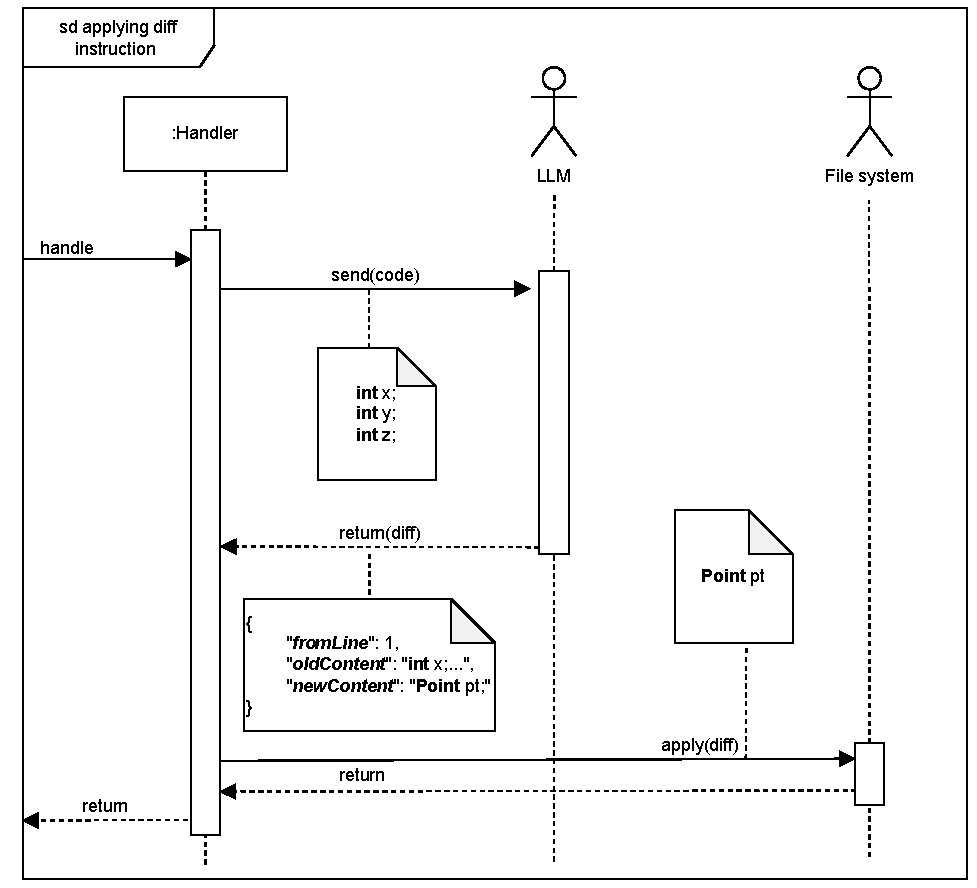
\includegraphics[width=1\columnwidth]{figures/chapter4/sequence_diagram_piece_output.drawio.pdf}
    \caption{\ac{UML} sequence diagram of applying a diff instruction (UML 2.5)}
    \label{fig:json_based_changes}
\end{figure}





One major issue is how to correctly apply the suggested changes if the model makes mistakes. 

Two approaches are possible.
In the first approach, the content at lines \textit{}{fromLine} to \textit{toLine} is replaced by \enquote{newContent}. This can be challenging if \enquote{newContent} has more lines than \enquote{oldContent}. Additionally, even if these  changes are correctly applied, later changes in the same file can become more problematic as the line number information might be outdated. 

Alternatively, a replacement method can be used. This means that the string \textit{oldContent} is replaced by \textit{newContent} without considering the line number information. This method prevents the issues of the first approach. Additionally, it might refactor more lines that the \ac{LLM} did not refactor for some reasons. This can have advantages but also challenges. For instance, an instruction to replace all curly brackets (\enquote*{\{}) by an empty string in a Java file can lead to non-compilable programs.  
Additionally, this does not work if \textit{oldContent} for some reason does not exist in the file. For instance, the model might have added extra whitespaces to the old content so that a simple search-and-replace-strategy does not work. Furthermore, if \textit{oldContent} is an empty string, replacing can lead to file corruption as the replacement operations are not developed for such an scenario. 

On the other hand, if multiple methods share the same parameters, the replace approach can change them all at once even if the output of the model does not suggest such changes. While adhering to the output of the \ac{LLM} is useful, it is restricted due to its output size limitations. Consequently,  this method can forestall incomplete refactoring. 

As a result, the decision which strategy to use is complex and can strongly impact the number of changes until the source code can build again. In general, the shorter the old content is, the more likely should the first approach be used, but exact criteria cannot be given. 


In this master's thesis both approaches are employed. The second approach is always tested first if the changes exceed a threshold of ten characters. If this approach does not work (e.~g. \enquote{oldContent} does not exist in the file, the line-by-line replacement method is used.  

\subsubsection{Handling invalid \ac{JSON} objects}

When using the \ac{JSON} output format, it is essential to deal with edge cases where the output is not valid \ac{JSON}. This problem can happen in two scenarios.

Firstly, not all \acp{LLM} support \ac{JSON}-only modes. This means that that the content of the model cannot be forced to contain only \ac{JSON} but might contain additional unparsable text that cannot be parsed. 

The model used in this thesis supports the \ac{JSON}-only mode. Nevertheless, it is still useful to keep these edge cases in mind. This edge case can be circumvented by finding the first opening curly brace \enquote{\{} in the response and the last closing curly brace \enquote{\}} because the string between should be valid \ac{JSON}. 
As a result, any text before or after the \ac{JSON} is ignored and cut off. 

Secondly, one problem for \acp{LLM} is that they generate token by token and therefore cannot pre-plan their output. Usually, this does not cause problems. 

However, as outlined in section \ref{sec:llm_challenges}, the maximum output size of a model is restricted so that a model cannot generate large output at once. The model can be prompted to continue the output, but this requires additional prompts. Additionally, these interim prompts must be combined into one so that they can parsed.

If the output format is \ac{JSON}, handling interruptions can become problematic because \ac{JSON} syntax requires a precise structure. For example, if the closing curly braces are missing, standard \ac{JSON} parsers will struggle to process the data and will typically generate an error. This strict syntactic requirement means that even minor deviations can disrupt \ac{JSON} data handling.

The easiest solution to this problem is to simply ignore the output as the response was invalid. 
However,  one can still try to parse the output as the incomplete \ac{JSON} might still contain relevant data (e.~g. refactoring instructions). While the refactoring is probably incomplete, it might be a good start and possible errors can be fixed in the validation step.


\subsection{Proposal handling}\label{sec:proposal_handling}

One issue that might occur while working with \ac{LLM} is that their output quality can vary. The same prompt can generate various outputs of which some might be useful and some are not useful. This, however, is also an advantage of \acs{LLM}. Refactoring data clumps can be performed in many different ways and therefore, the first output might not be the best output. 

Hence, a proposal system is useful where the model is asked multiple times for a solution to a query (e.~g. data clump refactoring). These proposals can be handled parallel or serial.  

\subsubsection{Parallel Proposals}
The model generates multiple independent proposals. This means that in each proposal the model has no memory of its previous proposals. At the end, the best proposal is chosen and applied to the source code.

The issue is to determine the \enquote{best} proposal. One approach could be to determine the proposal that causes the least compiler errors. While this idea might be helpful to reduce the manual work to correct errors, it also can tend to produce proposals that change as few code as possible. For instance, refactoring nothing can cause no compiler errors.

As an alternative, one could count the number of changed lines in a proposal and rate proposals with more changes higher than those with fewer changes. This idea rewards proposals that refactor all locations of interests more than proposals that only refactor only a small part of the program while the data clump exists in other known parts too. 


Another possible idea is to let the user decide. For instance, for each proposal, a new branch in the \ac{VCS} could be created so that a user can choose manually which version would be best one. After choosing a particular branch, the changes could be merged back to the original branch. Alternatively, an interactive dialog  could allow the user to zap through all proposals without changing branches. When selecting a proposal, the changes from the previous proposal are deleted and the new proposal is applied to the source code. However, this strategy requires active human intervention. 

This master's thesis does not attempt to explore which proposal selection strategy is suitable or whether other strategies would be better. 

\subsubsection{Sequential proposals}

With sequential proposals, one conversation is hold and the context is kept so that that the \ac{LLM} does not forget its previous output. Using this idea, not the first proposal is chosen but the last one after the \ac{LLM} has been given enough chances to correct errors.

Handling sequential proposal can be a combination of refactoring and validation handlers. At first, the usual refactoring process is performed. This could be a manual refactoring (e.~g. PSI) or a refactoring via an \ac{LLM}. Then, the refactored code is built. If there a building issues (e.~g. compiler errors or failing tests), the model is instructed to fix them. From now on, only the \ac{LLM} performs the refactoring even if a manual approach was used. Then, the code is built again, and the process starts again if there are errors. 



It should be noted that at some point a proposal should finally be chosen as the \ac{LLM} might not always find a solution that compiles even if infinitive steps were available. Similar to a an optimization algorithm, it can be struck into a local optimum and cannot suggest reasonable changes so that the program compiles again.  